%!TEX root = ../paper.tex

\subsection{Risk and Benefit Rankings} 
\begin{figure}[t]
	\centering
	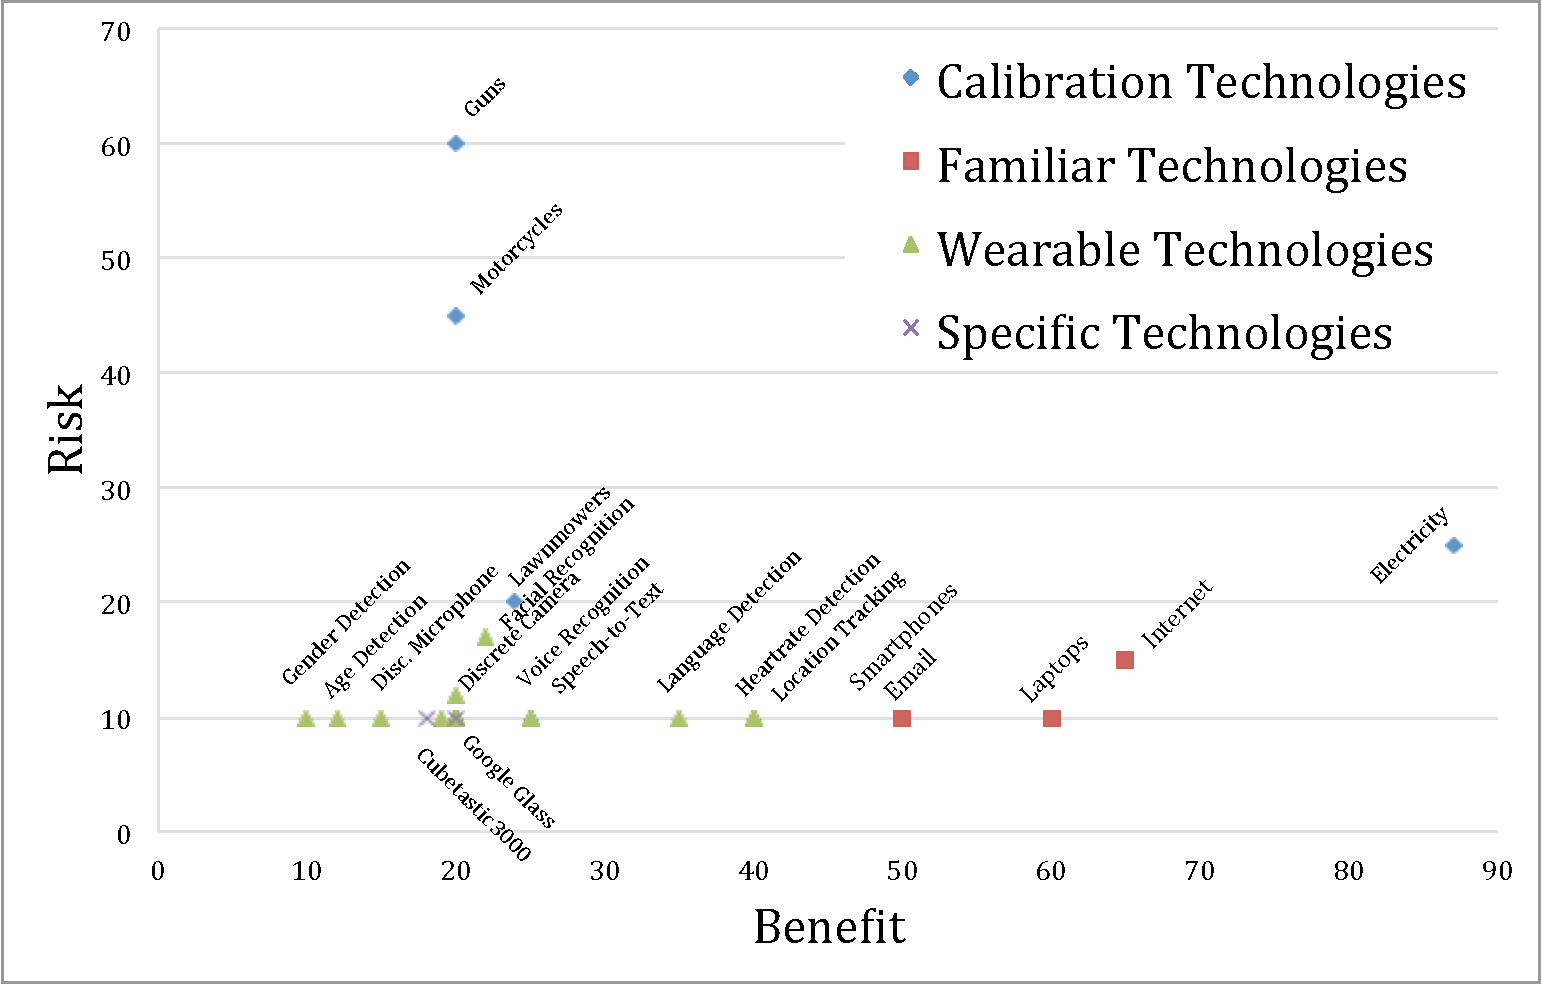
\includegraphics[width=0.47\textwidth]{images/riskbenefit.pdf}
	\caption{Participants' median risk-benefit ratings of technologies examined by Fischhoff \etal\cite{Fischhoff}, which we used for calibration, alongside familiar technologies (e.g., laptops, the Internet, etc.), wearable technologies, as well as two specific wearable devices (Google Glass and the Cubetastic3000).}
	\label{fig:techplot}
\end{figure}

We asked participants to rate new capabilities related to wearable technologies (e.g., facial recognition) in terms of their risks and benefits. We also asked them to do this for technologies with which they were likely to be more familiar (e.g., smartphones and laptops) in addition to two examples of specific wearable devices, Google Glass and the fictitious Cubetastic3000. To calibrate our results, we also asked about four well-established technologies studied by Fischhoff \etal\cite{Fischhoff}. We found that participants generally rated technologies related to wearables as being low-risk comparatively to other technologies (Figure \ref{fig:techplot}). Appendix ~\ref{sec:riskben-appendix} shows participants' median, quartiles, and distributions of risks and benefit ratings for all technologies. We found that the calibration technologies, which were more familiar to the participants, were all rated as the most risky. 

As a group, participants rated more familiar technologies as the more beneficial. We believe this is the result of exposure people have to these technologies---most people use these technologies daily and therefore see what the benefits of these technologies are. It is true that people perceive unfamiliar technologies as less beneficial at the moment, but this will change as the use of these technologies evolve and adoption increases. Most calibration technologies, with the exception of electricity, were seen as lower benefit than the others. However, Google glass and Cubetastic3000 were about equally beneficial, and gender and age recognition were less beneficial. 

Of the wearable technologies, privacy-invasive ones were perceived to be risky. Top risky technologies include facial recognition, the Internet, and discrete cameras, whereas the remainder of the technologies were seen as having minimal,  equivalent risk levels (i.e., a median of ``10''). The differences in risk that found between the different wearable-related technologies, are not tested for statistical significance, but given their minimal spread compared to the calibration options, the differences are negligible. Interestingly, privacy risks and are comparative to real physical risks; for instance, the capacity for facial detection on a wearable device is perceived to be almost as risky as interacting with a lawnmower. 

People prompted to rate with respect to all considerations (see ~\ref{sec:prompt}), including physical harm risk to bystanders, financial cost, distress, misuse, or impact on public, personal, and private life, people may have still evaluated the risks with an emphasis toward physical risk and without an emphasis on privacy risk. Among the 5 presented options, the wearable-related one is the only one without some physical risk scenario, and physical risk is a clear, tangible risk to the users. 

These perceptions of the most risky or beneficial technologies may not be reflective of actual risks or benefits. However, they do reflect the general public's exposure to these technologies and show that people perceive specific risks and benefits. We suspect that the similarity in assessments between the various wearable technologies are because most people are not consciously aware of the possibilities of these technologies or how they could be used. We suspect that performing this experiment longitudinally may yield more interesting results, as these technologies become more and more pervasive (and therefore more familiar to participants).